\chapter{Experiment on spawn points placement heuristics}

% INTRODUCTION %

In this chapter we describe the experiment that we have performed for validating the placement heuristics for spawn points described in the previous chapter and, at the same time, for testing the data-collection capabilities of our framework, that was used to setup and manage the experiment.

% DESCRIPTION %

\section{Description}

With this experiment we analyzed how the placement of spawn points influences the up-player vs down-player dynamic. The experiment tries to recreate the situation where the up-player, once killed his opponent, tries to find him as soon as possible, just after his respawn, to score another easy kill. As we have seen, a well-designed map should slow down this operation by having its spawn points in areas that are not central, are easy to leave and covered. The \<low risk> heuristic described in chapter \ref{sss:lowrisk} has been designed to place the spawn points according to such criteria, so, to prove its effectiveness, we decided to confront how this facet of the up-player vs down-player dynamic changes with respect to spawn points placed with the \<uniform> heuristic, defined as well in chapter \ref{sss:uniform}, which selects the areas to contain spawn to be distributed evenly inside the map.

\par

To highlight this particular dynamic, we designed a game mode where the user, which represents the up-player, must find and destroy a static target, which represents the down-player, as many times as possible before times runs out. Each time that the user destroys a target, it respawns at a random spawn point. The user cannot die and has infinite ammunition, so he does not have to look for resources.

% SETUP %

\section{Setup}

For this experiment, we setup the \<Experiment Manager> to propose in each play session a quick tutorial, two matches and a survey. The experiment was composed by three \<studies>, corresponding to different pre-generated maps, each one composed by two \<cases>, one that corresponded to the \<low risk> spawn points distribution and one that corresponded to a pool of five \<uniform> spawn point distributions. In a play session, the user played the same map twice, once with the low risk distribution and once with one of the uniform distributions, in a random order and with the map flipped in one of the two matches. We used the survey to profile how much the user was familiar with video games and FPS, to evaluate his skill and to get a feedback about in which of the two maps it was harder to find the targets. The experiment was deployed online and played by the users via browser on their own computer.

\par

Each match had \<Target Hunt> as game mode. The duration of the match was set to three minutes, the list of spawnable entities consisted of just one target and the only weapon available to the player was the \<assault rifle> with infinite ammunition. The pre-generated maps were stored as text files and were loaded by the \<Divisive Generator> and displayed with the \<Prefab Assembler>. 

\par
 
For each match, a complete game log was saved, along with the following performance metrics, saved in a separate log:
 
 \begin{itemize}
\item \<TargetLogs>: this field contains a list of all the targets that the user managed to destroyed. Each entry contains a timestamp of when the target was destroyed, the coordinates of the target, the coordinates of the user, the distance covered by the user and the time passed during the lifespan of the target.
\item \<Shots>: the total number of projectiles shot by the user.
\item \<Hits>: the number of projectiles that hit a target.
\item \<Accuracy>: the percentage of projectiles that hit a target.
\item \<Kills>: the total number of targets destroyed by the user.
\item \<Distance>: the total distance covered by the user during the match, considering cells of unitary width.
\item \<AvgKillTime>: the duration of the match divided by the number of kills.
\item \<AvgKillDistance>: the total distance divided by the number of kills.
\end{itemize}

\noindent
The answers to the survey were saved as well.
 
 \par
 
The performance of the player is measured by \<AvgKillTime>, that is also an indicator of how difficult it is to find targets in the map.

\par
  
We have selected three procedurally generated maps that present radically different layouts and we populated each one of them using both the low risk and the uniform heuristic:

\begin{itemize}
\item \<Arena>: this map presents a wide open arena, two sides of which are adjacent to parallel corridors with many openings. As the visibility heatmap in figure \ref{img:arena_visibility} shows, the central arena allows to control most of the map, whereas the corridors offer some repair and perfect spots to place spawn points. Figure \ref{img:arena_safe} shows the spawn points positioned using the low risk heuristic, whereas figure \ref{img:arena_uniform} shows one of the five configuration produced using the uniform heuristic.
\item \<Corridors>: this map presents many small rooms connected by long corridors. As it can be seen in figure \ref{img:corridors_visibility}, there is no area that allows to control the others and the only point with high visibility are the ones where corridors intersect. Figure \ref{img:corridors_safe} shows the spawn points positioned using the low risk heuristic, whereas figure \ref{img:corridors_uniform} shows one of the five configuration produced using the uniform heuristic.
\item \<Intense>: compared to the previous two, this map presents an intermediate layout, since it has both open areas and small rooms connected by corridors. As it can be seen in figure \ref{img:intense_visibility}, this reflects also on the visibility, that is high in the central open arenas and low in the remaining sections of the map. Figure \ref{img:intense_safe} shows the spawn points positioned using the low risk heuristic, whereas figure \ref{img:intense_uniform} shows one of the five configuration produced using the uniform heuristic.
\end{itemize}

\par

It is important to observe that the low risk and the uniform heuristics select rooms to place a spawn point with two different criteria, but they employ the same logic when selecting a tile inside a room. This means that the two heuristics select tiles which have similar visibility conditions, so the player's performance difference depends exclusively on how the rooms have been selected. This is observable in figures \ref{img:arena}, \ref{img:corridors} and \ref{img:intense}: when the uniform heuristics happens to select a room that has been selected also by the low risk one, the spawn point is placed exactly on the same tile.

\begin{figure}[tp]
	\centering
	\begin{subfigure}[t]{0.3\linewidth}
    		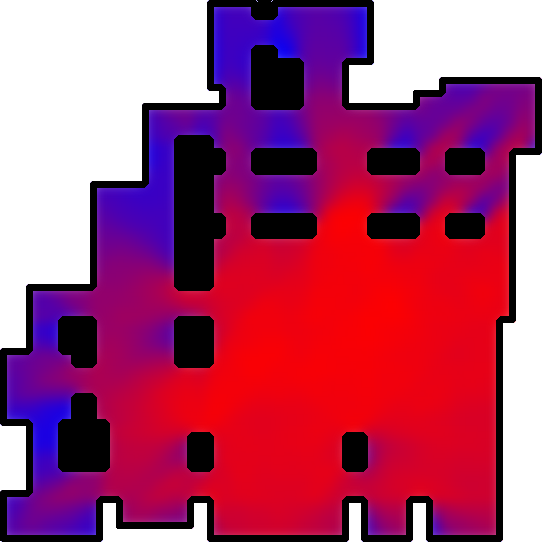
\includegraphics[width=\linewidth]{arena_visibility}
     		\caption{Heatmap showing the visibility of the level.}
		\label{img:arena_visibility}
  	\end{subfigure}  	
  	\hfil
  	\begin{subfigure}[t]{0.3\linewidth}
    		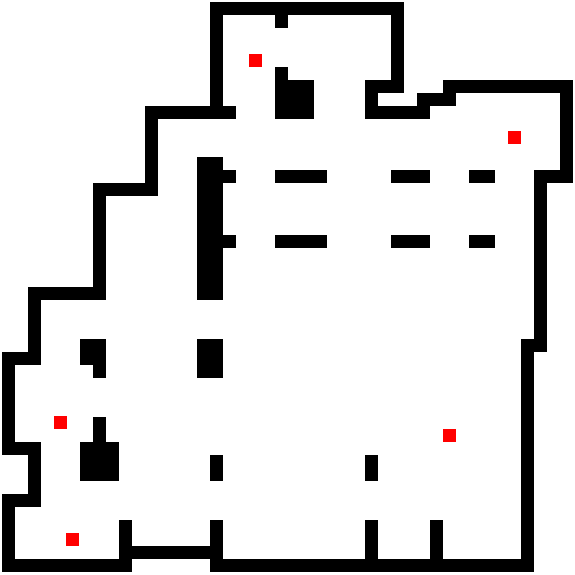
\includegraphics[width=\linewidth]{arena_safe}
     		\caption{Spawn points (in red) placed using the safe heuristic.}
     		\label{img:arena_safe}
  	\end{subfigure}
  	\hfil
  	\begin{subfigure}[t]{0.3\linewidth}
    		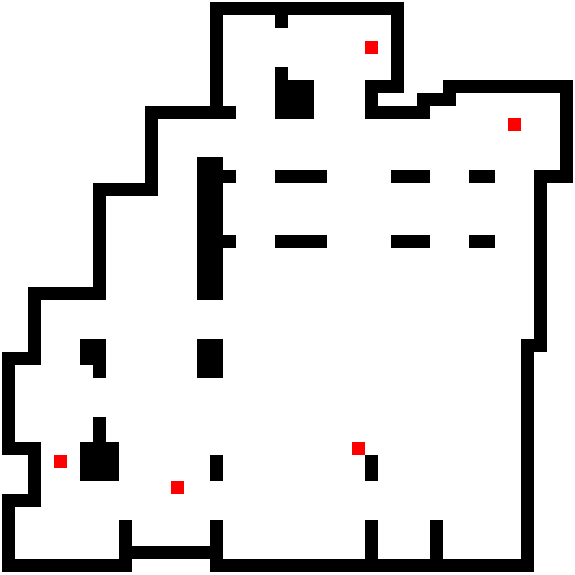
\includegraphics[width=\linewidth]{arena_uniform}
     		\caption{Spawn points (in red) placed using the uniform heuristic.}
		\label{img:arena_uniform}
  	\end{subfigure}  
	\caption{``Arena'' map used in the experiment.}
	\label{img:arena}
\end{figure}

\begin{figure}[tp]
	\centering
  	\begin{subfigure}[t]{0.3\linewidth}
    		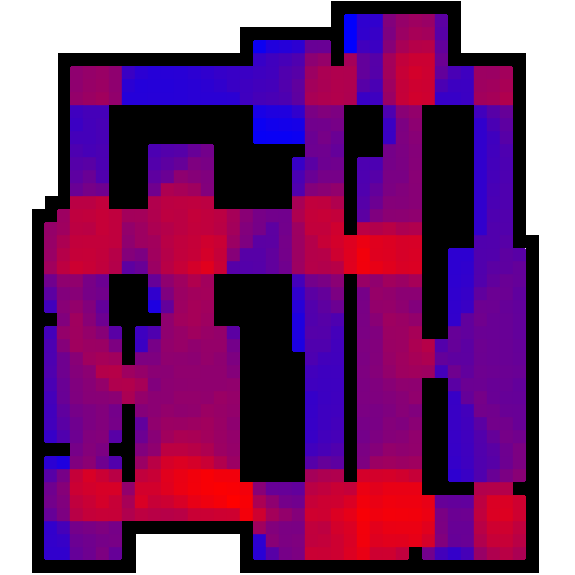
\includegraphics[width=\linewidth]{corridors_visibility}
     		\caption{Heatmap showing the visibility of the level.}
		\label{img:corridors_visibility}
  	\end{subfigure}  	  
  	\hfil
  	\begin{subfigure}[t]{0.3\linewidth}
    		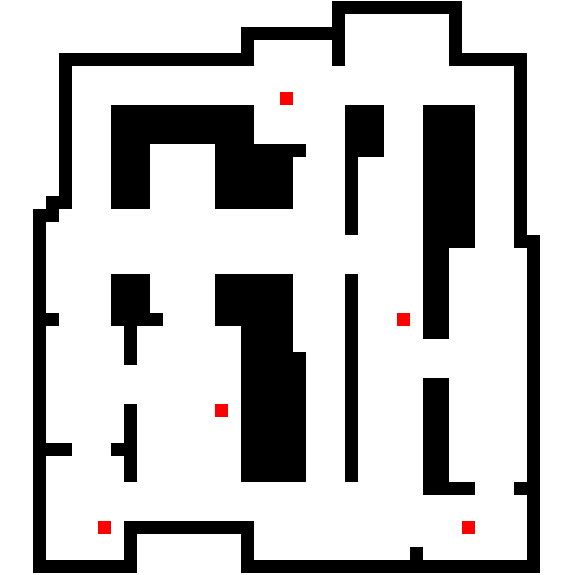
\includegraphics[width=\linewidth]{corridors_safe}
     		\caption{Spawn points (in red) placed using the safe heuristic.}
     		\label{img:corridors_safe}
  	\end{subfigure}
  	\hfil
  	\begin{subfigure}[t]{0.3\linewidth}
    		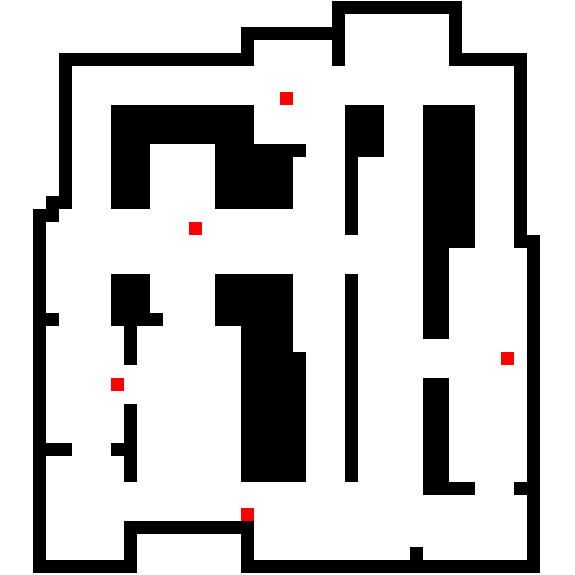
\includegraphics[width=\linewidth]{corridors_uniform}
     		\caption{Spawn points (in red) placed using the uniform heuristic.}
		\label{img:corridors_uniform}
  	\end{subfigure}	
	\caption{``Corridors'' map used in the experiment.}
	\label{img:corridors}
\end{figure}

\begin{figure}[tp]
	\centering  	
  	\begin{subfigure}[t]{0.3\linewidth}
    		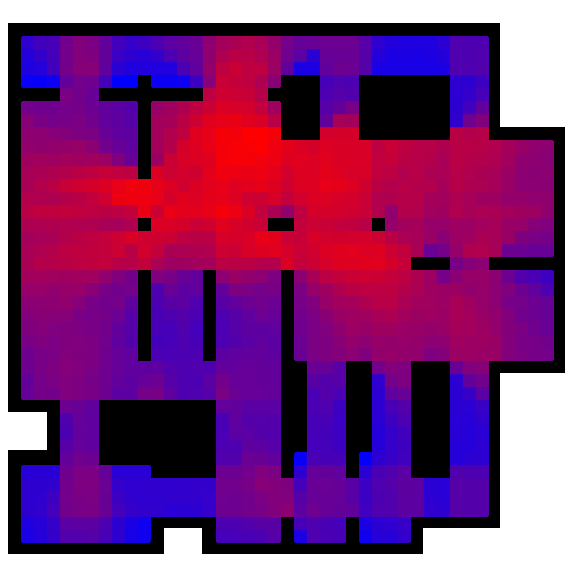
\includegraphics[width=\linewidth]{intense_visibility}
     		\caption{Heatmap showing the visibility of the level.}
		\label{img:intense_visibility}
  	\end{subfigure}  	
  	\hfil
  	\begin{subfigure}[t]{0.3\linewidth}
    		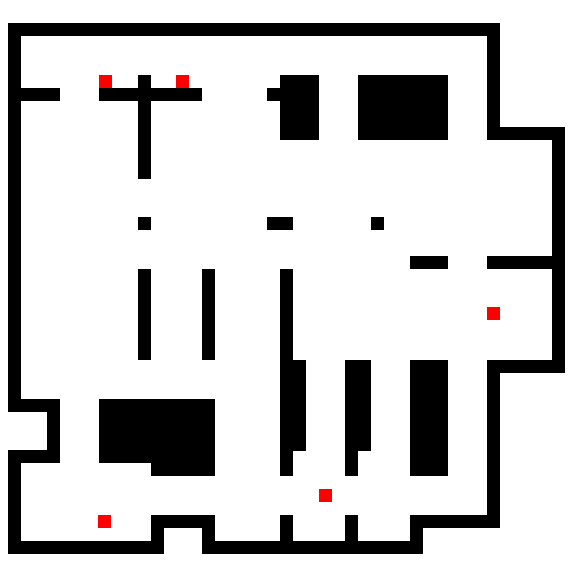
\includegraphics[width=\linewidth]{intense_safe}
     		\caption{Spawn points (in red) placed using the safe heuristic.}
     		\label{img:intense_safe}
  	\end{subfigure}
  	\hfil
  	\begin{subfigure}[t]{0.3\linewidth}
    		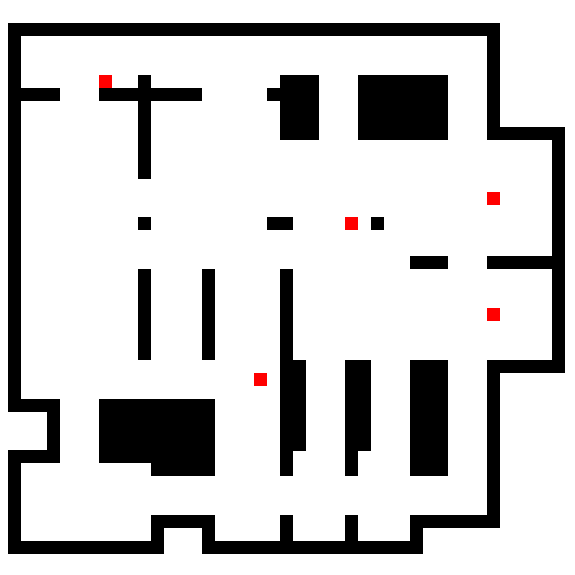
\includegraphics[width=\linewidth]{intense_uniform}
     		\caption{Spawn points (in red) placed using the uniform heuristic.}
		\label{img:intense_uniform}
  	\end{subfigure}
	\caption{``Intense'' map used in the experiment.}
	\label{img:intense}	
\end{figure}

% RESULTS %

\section{Results}

\begin{figure}[tp]
 	\centering
  	\begin{subfigure}[t]{0.8\linewidth}
    		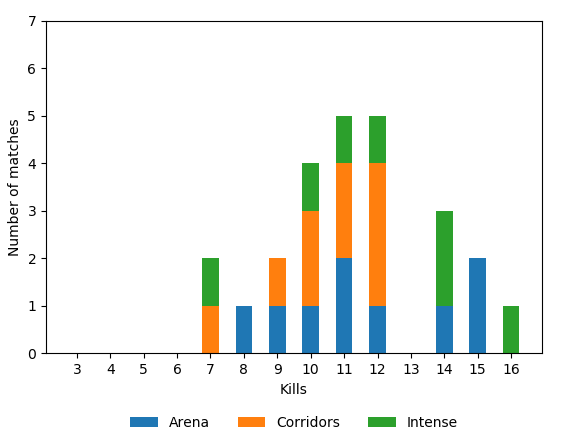
\includegraphics[width=\linewidth]{bar_lowrisk}
     		\caption{Low risk heuristic.}
		\label{img:bar_lowrisk}
  	\end{subfigure}  	
  	\begin{subfigure}[t]{0.8\linewidth}
    		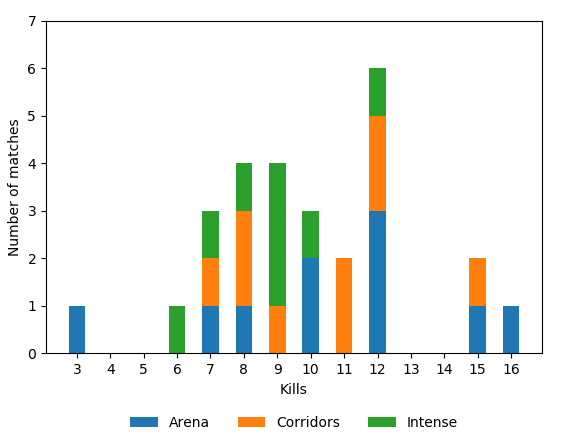
\includegraphics[width=\linewidth]{bar_uniform}
     		\caption{Uniform heuristic.}
     		\label{img:bar_uniform}
  	\end{subfigure}
	\caption[Distribution of the matches by number of kills for the two heuristics.]{Distribution of the matches by number of kills for the two heuristics. The matches are also classified by map.}
	\label{img:match_distribution}	
\end{figure}

\begin{figure}[tp]
 	\centering
  	\begin{subfigure}[t]{0.48\linewidth}
    		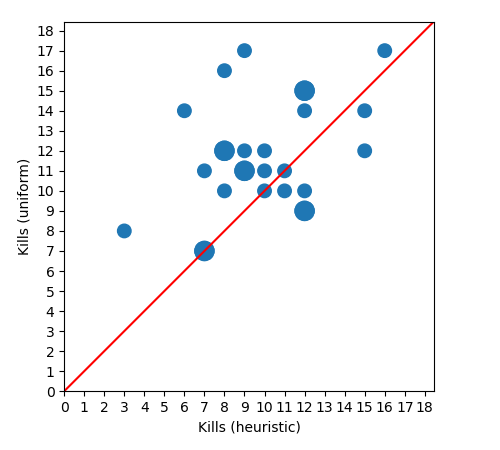
\includegraphics[width=\linewidth]{scatter_kills}
     		\caption{Kills.}
		\label{img:bar_lowrisk}
  	\end{subfigure}
  	\hfill
  	\begin{subfigure}[t]{0.48\linewidth}
    		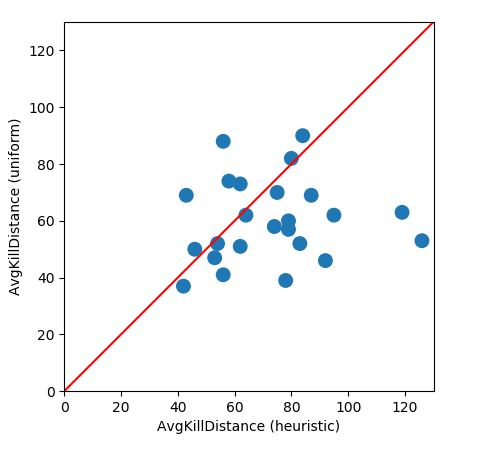
\includegraphics[width=\linewidth]{scatter_avg}
     		\caption{AvgKillDistance.}
     		\label{img:bar_uniform}
  	\end{subfigure}
	\caption[Experiment outcomes by metrics.]{Experiment outcomes by metrics. The outcome associated to the low risk heuristics is on the horizontal axis, the one associated to the uniform heuristics is on the vertical axis.}
	\label{img:metrics}	
\end{figure}

\begin{figure}[tp]
 	\centering
	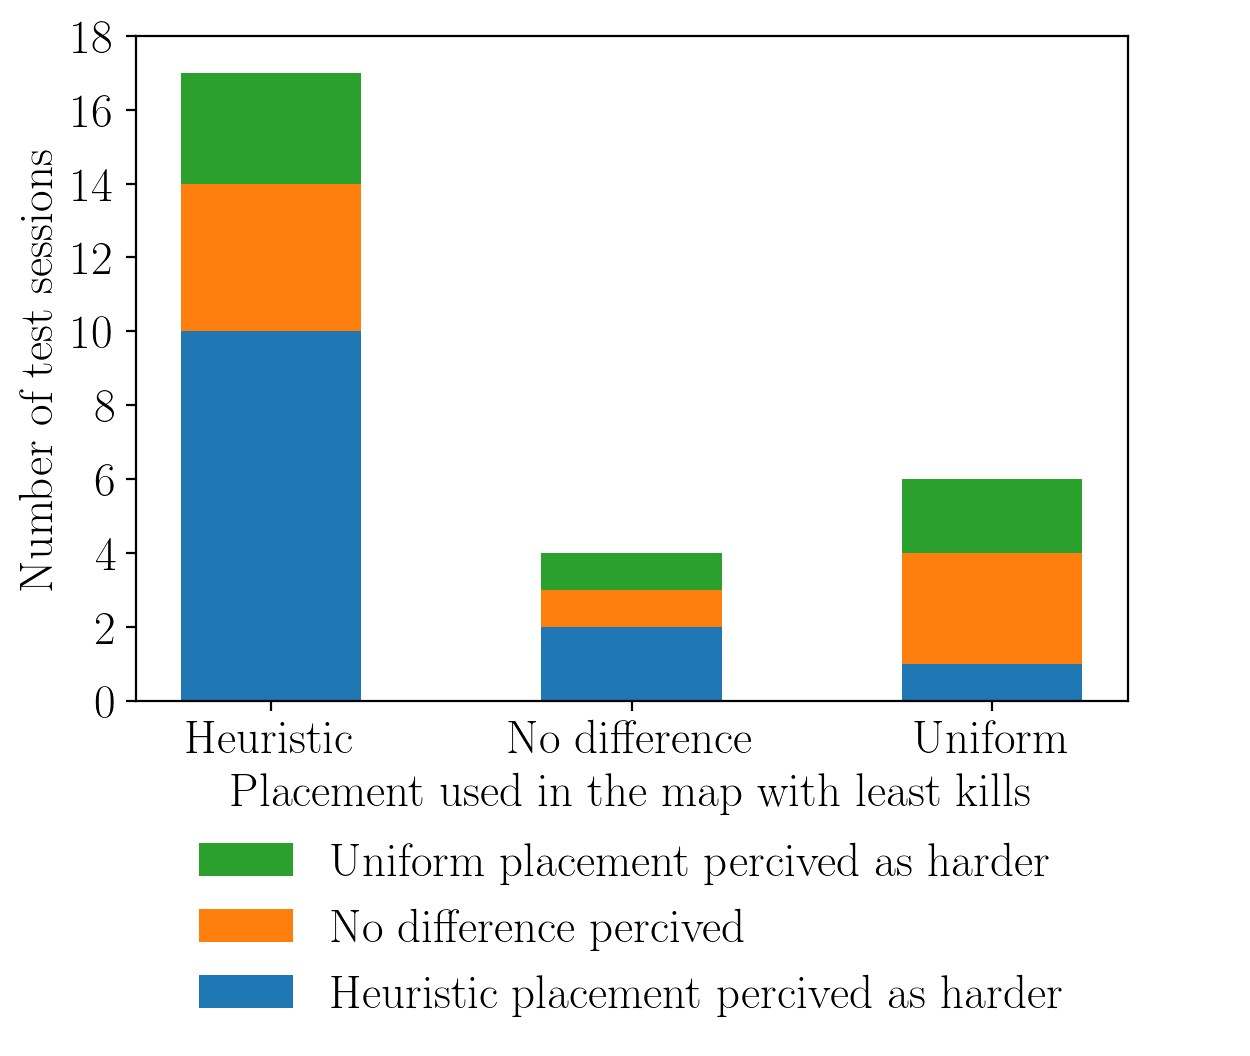
\includegraphics[width=0.8\linewidth]{percived}
	\caption{Comparison between the effective and the perceived difficulty.}
	\label{img:percived}		
\end{figure}

% CONCLUSIONS %

\section{Conclusions}

